Một học sinh được giao nhiệm vụ chế tạo một kính thiên văn đơn giản từ những dụng cụ tại gia. Thật may mắn, bố của cậu học sinh là chủ một xưởng sản xuất gia công mài tiện thuỷ tinh, quyết định giúp con trai của mình tạo ra ba thấu kính hội tụ để tạo một chiếc kính thiên văn khúc xạ đơn giản có những thông số tiêu cự-đường kính như sau
\begin{itemize}\itemsep0em
\item \eqmakebox[things][l]{Vật kính: }
     $ \begin{aligned}[t]
      F = 1200 \mathrm{~mm}\\
      D = 130 \mathrm{~mm}
      \end{aligned} $
\item \eqmakebox[things][l]{Kính trường: }
     $ \begin{aligned}[t]
      f_0 = 45 \mathrm{~mm}\\
      d_0 = 30 \mathrm{~mm}
      \end{aligned} $
\item \eqmakebox[things][l]{Kính mắt: }
     $ \begin{aligned}[t]
      f= 15 \mathrm{~mm}\\
      d = 15 \mathrm{~mm}
      \end{aligned} $
\end{itemize}

Thứ tự lắp đặt như sau: $\text{Vật kính} \rightarrow \text{Kính trường} \rightarrow \text{Kính mắt}$, được đặt đồng trục. Mục đích của kính trường là để tăng thị trường nhìn của kính thiên văn. Thực tế các thị kính kính thiên văn chuyên nghiệp trên thị trường hiện nay bao gồm ít nhất hai thấu kính thành phần. Thị kính tự chế này có hai thấu kính trường và thấu kính mắt đặt cách nhau một khoảng $l = 30 \mathrm{~mm}$. Biết mắt ngắm chừng ảnh ở vô cực. Sơ đồ kính thiên văn tự chế (Hình vẽ không đúng tỉ lệ).
\begin{figure}[h!]
    \centering
    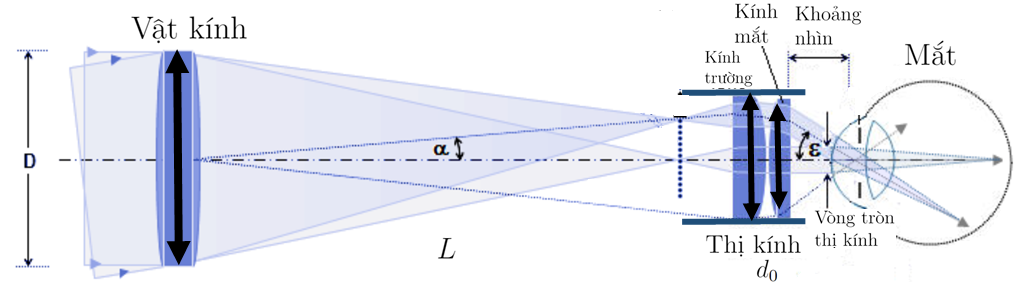
\includegraphics[scale=0.5]{Problem_4/P4.png}
    \label{fig_P4}
\end{figure}

\vspace{1cm}

\textbf{1.} Hãy xác định:
\begin{enumerate}[label=\textbf{\alph*,}]\itemsep0em
\item Khoảng cách giữa vật kính và kính trường theo $F, f, f_0, l$.
\item Độ bội giác của kính thiên văn theo $F, f, f_0, l$.
\end{enumerate}

\textbf{2.} Để mắt nhận được toàn bộ ánh sáng từ việc quan sát, người ta đặt mắt ra xa kính mắt một khoảng $\Delta$. Tức là khi đó \textit{ảnh của vật kính} nằm trên mắt. Biết đồng tử mắt có đường kính khoảng 7 mm. Hãy xác định $\Delta$ và đường kính vòng tròn ảnh vật kính trên mắt khi đó, biến đổi $\Delta$ theo dạng
$$\Delta = f\left(a + \frac{f}{F} b \right). $$
Xác định $a$ và $b$ theo $F, f, f_0, l$. Hỏi mắt người có nhận được toàn bộ ánh sáng không?

\vspace{1.5mm}

\textbf{3.} Đặt mắt cách kính mắt khoảng $\Delta = 5 \mathrm{~mm}$. Biết Mặt Trăng có bán kính là $R_M = 1737.4 \mathrm{~km}$ và cách Trái Đất $d_{ME} = 384400 \mathrm{~km}$. Hãy xác định xem bao nhiêu phần trăm diện tích ảnh của Mặt Trăng qua kính thiên văn xuất hiện trên vùng ta quan sát? % (\textit{Không nên biến đổi tổng quát, hãy \textbf{thay số!!}})

\begin{flushright}
    (Biên soạn bởi Zinc)
\end{flushright}